%%% Made of Tiny Robots
%%% An Investigation of the Ecology of Responsive Environments
%%%
\chapter{Introduction}
\label{ch:intro}
%
What follows is an investigation into the ways the burgeoning \textbf{ubiquity of computation}%
\footnote{Terms rendered in bold on first use are defined in the Glossary.}%
\footnote{A trend identified by Weiser \citeyearpar{weiser_1999}.}
will reshape the way we relate to our physical environment.
Putting computers and screens and sensors and networking and even motors in artifacts whose utility was previously primarily conferred by their physical form will give the artifacts in our environment internal states and behaviors; our physical environment will become responsive.
In the extreme case of artifacts composed of \textbf{self-reconfiguring materials} the form of an artifact will become just another aspect of its behavior.
This change from form-governed artifacts (where an artifacts's utility is conferred by its form) to behavior-governed artifacts (where an artifacts's utility is conferred by its behavior) is the hallmark of a \textbf{responsive environment}.
Thus in a responsive environment our role shifts from being the sole actors who make use of the tools we surround ourselves with to being (perhaps leading) members of a social network of robotic%
\footnote{We will be considering \textbf{robots} in the broadest possible sense of any machine capable of sensing input and responding with various behaviors.}
artifacts.

We suggest that taking an ecological perspective is important to understanding the shift to responsive environments for two reasons:
\begin{enumerate}
\item these networked robotic artifacts will serve as cybernetic extensions of our capabilities, and the level of the interface will be ecological; and
\item the complexity of producing these artifacts combined with their intimate connection with and knowledge of our personal lives will change the dynamics of their production, distribution and use.
\end{enumerate}
To be clear, when we speak of ecology we do not intend it in the sense of the natural environment.
We will be investigating \textbf{artifact ecologies}, the systems we apply and roles we adopt in the creation and use of physical artifacts, and the network of relations thus engendered.

In the rest of the introduction we further elaborate on the evolution of artifact ecologies, how we will interface with responsive environments composed of robotic artifacts, and the roles we will adopt in creating and customizing these new robotic artifacts.
We then argue that one of these ecologies is particularly well suited to engaging communities in specifying the behavior of their responsive environments, and outline how the following chapters will develop and support this claim.

\section{The Evolution of Artifact Ecologies}
%
To understand the manner in which we are embedded in ecologies of the creation, distribution and use of artifacts we need a theory of how we relate to individual artifacts.
Gibson \citeyearpar{gibson_1979} suggests that we are able to appreciate the value of physical artifacts through our (innate) recognition of the uses \textbf{afforded} by their form.
We recognize without effort that a chair affords the possibility of sitting and a door in a wall affords the possibility of entering a building. 

We propose that the history of artifact ecologies consists of two broad eras, and we are now on the cusp of a third era.

As our (primate) ancestors developed the faculties to recognize that, for example, flint could be knapped to produce a blade, which could then be used to skin animals to create clothing, we entered the first era of the \emph{wild environment}%
\footnote{Terms coined here are emphasized on first use, and defined in the Glossary.}. 
These sorts of artifact ecologies are characterized by a distinction between a local collection of useful artifacts with clear affordances, generally carried on one's person, and a vast external environment that does not particularly respond to the human scale and within which affordances can be perceived only with significant knowledge and effort.
Artifacts are generally crafted by the bearer for personal use from raw materials harvested from the wild surroundings. 
The chief social aspect of these artifact ecologies was the verbal transfer of the relevant methods to close acquaintances.

The next era was ushered in by the development of urban settlements. 
In these \emph{leveraged environments} our artifact ecology has expanded to the horizon; we are now surrounded by manufactured artifacts designed to present a variety of helpful affordances.
These artifacts give us leverage over our local conditions, for example doors allow us to easily restrict access to a space.
Artifacts are no longer simply controlled by their bearer and encode complex social dynamics; roads and sidewalks are shared by citizens, stores provide artifacts in exchange for money, doors open for those who bear their keys.
In order to produce these new artifacts in sufficient quantity to literally pave over the natural environment significant social changes are required; artifacts are designed by one set of specialists, produced by another, and distributed by yet another.
As desirable artifacts are mass-manufactured through a complex bureacracy they are frequently unevenly distributed.
The artifact ecologies of this era frequently engender social unrest due to inequities in the control of public artifacts and the distribution of private artifacts.

Many people already carry small computational devices with them and routinely interact with these newly familar robotic interfaces. As this computational ubiquity spreads we are already transitioning into a third era of artifact ecologies: responsive environments. These ecologies will be characterized by the promotion of our artifacts from passive tools to networked social peers. The intimacy of these relationships will place much more power over our behaviors and emotions in the hands of those who dictate the behavior of these artifacts. At the same time these artifacts have the potential to allow mass customization to the desires of those bearing a given artifact. 

\section{Where Do We Plug In?}
%
Science fiction stories have led many people to ask: (when) will we have computer chips in our heads?%
\footnote{I am indebted to William Gibson \citeyearpar{gibson_distrust} for this formulation.} 
The answer for most of us is probably never, as we do not actually need to cut into our brains to become \textbf{cyborgs}; we are fully capable of interfacing with computers through language, through \textbf{GUI interfaces} and through \textbf{tangible interfaces}.
By embedding ourselves in artifact ecologies populated with robotic devices with these sorts of interfaces, we in effect incorporate these other computational systems into our own thought processes.
The best current example of this kind of cybernetic interface is \textbf{googling}; once one learns basic techniques for interacting with internet search engines and acquires a persistent network interface (such as a \textbf{smart phone}%
\footnote{While this term is currently well known we expect that in the near future it will seem as antiquated as ``personal digital assistant''.}%
) one becomes a sort of information-retrieval cyborg.
The googlebot is so easily incorporated into our minds because our minds are already just a collection of specialized computational units that in concert to form a ``society of mind'' \citep{society_of_mind}. 
As the philosopher of mind Daniel Dennett is fond of saying, ``Yes we have a soul; but it's made of lots of tiny robots'' \citeyearpar[][p. 1]{freedom_evolves}. Although these tiny robots have historically happened to all be in our brains, with the advent of responsive environments we will be incorporating more and more robotic devices into our local cybernetic artifact ecologies.

Many of these devices constantly feed data to apparently discorporate%
\footnote{The googlebot actually has a physical stature in line with its apparent omniscience; it fills several enormous buildings spread around the world and consumes enormous amounts of energy from both the grid and dedicated power plants.}
agents like the googlebot.
As we enter into a cybernetic relationship with this new artifact ecology much of what we have until now considered our private personas will be determined by the behavior of the robotic devices we surround ourselves with, and by our relationship with the computational agents that manage these devices and mediate our interactions with other people. 
In light of our special relationship we will refer to these agents (like the googlebot) generally as \emph{idols}%
\footnote{We chose the name `idol' after Gibson's `idoru'\citeyearpar{gibson_idoru}, a literal AI rock star, with the accompanying cultural leverage of a teen idol; and after religious idols, to draw an analogy with the religious practice of asking powerful ethereal agents for advice and favors.}.
We will call the handheld computers (such as a smartphone) that allow us to communicate with both peers and idols (through a constant connection to the network), \emph{crystals}%
\footnote{As in a crystal ball that is used to view distant places and communicate with other agents through the ether, and as a reference to their current popular physical realization as a fragile glass-plated touchscreen.}.

\section{New Materials}
%
While the heralds of responsive environments have been computers that will fit in your pocket, and interface with us through language and images, embedded computation has the potential to create artifacts that are much less familiar.
Computation is coming out from behind a screen and into the physical objects in the world around us. These robotic artifacts may respond to being touched and manipulated, or may proactively reconfigure the spaces around us.

\textbf{Tangible interfaces} give us the opportunity to leverage our innate recognition of the uses afforded by different forms. 
Physical kits that can be used to describe forms and concepts predate responsive devices. Educators have developed a variety of such physical kits known collectively as \textbf{manipulatives}. 
Tangible interfaces---by enhancing manipulatives with embedded computation---tie digital models to physical objects to allow people to directly grasp and manipulate these models \citep{tangible_bits}.
For example, our Posey kit allows people describe a 3D model to a computer by building it with a hub-and-strut construction kit rather than using an onscreen mouse-and-keyboard interface to manipulate graphical representations of shapes.

Tangible interfaces' physicality provides several inherent advantages: the physical system provides a representation of its own state \citep{jacob_chi2008}; physical constraints can enforce the constraints of the digital model \citep{patten_chi2007}; the \textbf{sensorimotor} feedback provided by manipulating physical objects helps to \textbf{scaffold} geometry and symbol manipulation tasks \citep{nesta_tangible_learning}; and several people can collaborate to provide input \citep{handsaw,algoblock}.

Traditional manipulatives are also the basis for \textbf{modular robotics} \citep{yim_ra2007}, which add computation and actuation to create kits of parts for quickly assembling robotic devices. 
(We will refer to these robotic devices assembled to perform a particular task as \emph{golems}%
\footnote{After the mythological golem assembled from clay to do its master's bidding.}.) 
By combining modular robotics and tangible interfaces, these golems can be programmed by directly manipulating them to demonstrate desired behaviors.

Making things---giving objects form---has traditionally involved a manufacturing process such as machining a block of material or pouring molten material into a mold. 
Recently, the techniques of modular robotics have been extended further to create a new kind of material that can receive a digital description of a desired form and arrange itself into that shape. 
One implementation of such a self{}-reconfiguring material is an \textbf{ensemble} of robotic modules. 
Each module runs a small program; together the programs encode the ensemble's behavior. 
By coordinating with neighbors, modules respond to external stimuli and arrange themselves into a potentially vast number of forms.

Self{}-reconfiguring materials promise to revolutionize the creation and distribution of physical objects much as digital audio files have revolutionized the distribution and content of music. 
The digital description of a chair or a bottle opener could be downloaded and then realized from a reservoir of self{}-reconfiguring material. 
Unused objects return to this reservoir to provide raw material for other objects.

More significantly, an object composed of this new material need not be limited to a single static form. 
Instead, the currently running program can change its form. 
We call a form that varies in the four dimensions of space and time a \emph{hyperform}; a single hyperform expresses itself as different shapes at different times.  
A new hyperform is realized just by loading a new program into the material. 
For example, the `social table' hyperform (Fig~\ref{fig:social_table}) automatically expands as more people sit down. 
The table grows to make space for additional guests (drawing more material from a household reservoir as needed); as people get up from the table after dinner, the social table melts away leaving only a small dinette with a single empty chair. 
The material that had been part of the expanded table returns to the reservoir and later renders a sofa and coffee table for guests to relax after dinner.

\begin{figure}[tb]
  \centering
    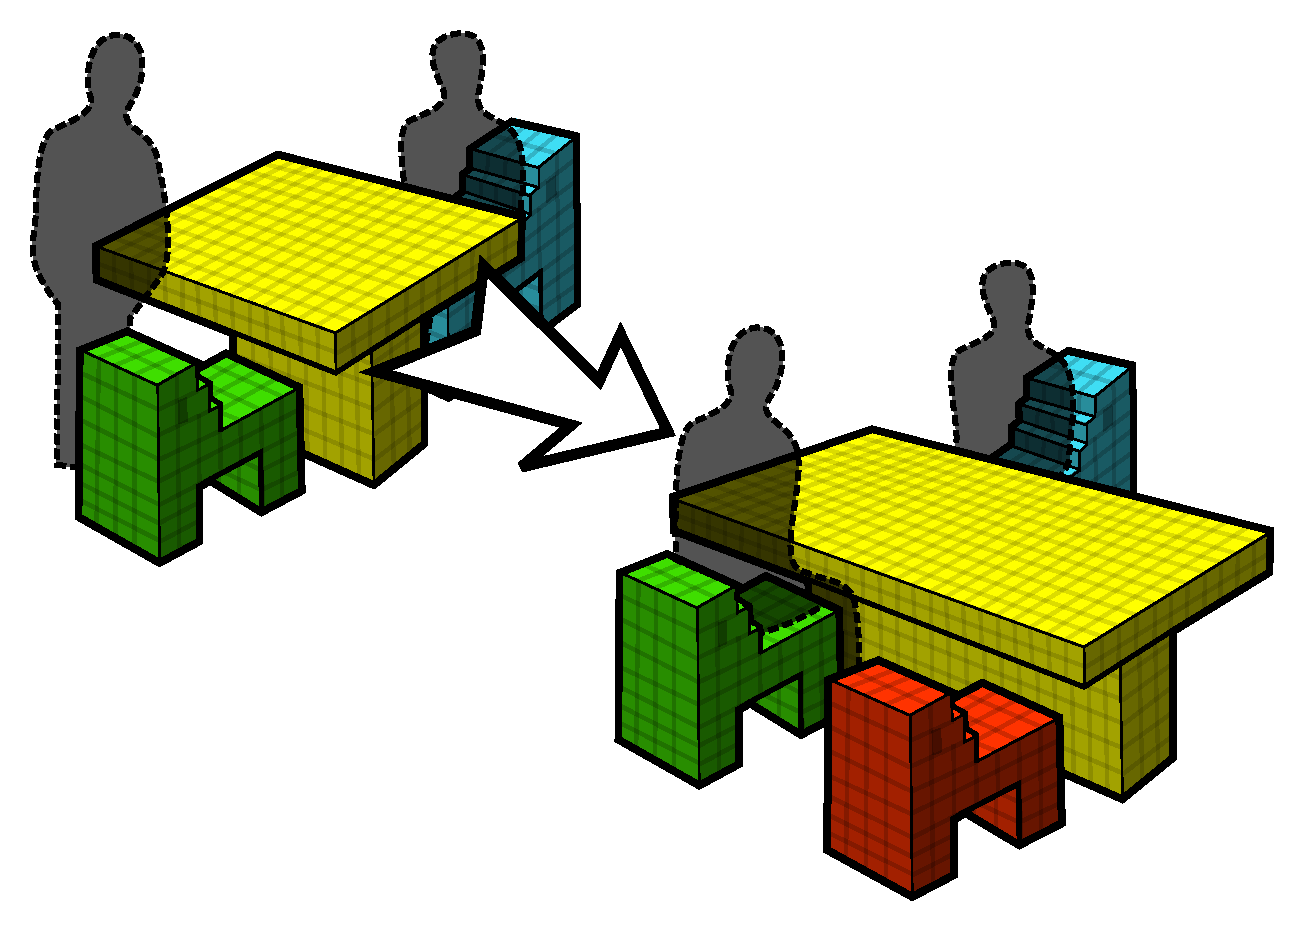
\includegraphics[width=100mm]{social_table.pdf}
  \caption{The social table, an example of a hyperform composed of self-reconfiguring robotic modules. As more people sit down, the table expands (drawing from a reservoir of modules) to keep one empty seat available.}
  \label{fig:social_table}
\end{figure}

Research towards even more advanced hyperform mediums is also underway. One vision is that a \textbf{claytronic} \citep{goldstein_computer2005} material could be composed of robotic particles (we will call them \emph{clayticles}) so small%
\footnote{Individual clayticle modules are less than 1mm in diameter. 
They are fabricated using the same processes used to make microchips, except that they are designed to curl up into a ball when they are released from their substrate.
Electronic actuators etched into their surfaces allow these tiny spheres to attach to each other and to self{}-reconfigure. (TODO: citation)}
that objects formed from the material appear to be molded out of clay rather than constructed out of blocks.

\section{Tiny Robots}
%
A particularly interesting subset of responsive artifacts are those systems extending traditional manipulatives with embedded computation.
These tiny robotic modules can serve as design interface, cybernetic cognitive enhancement and implementation medium all at the same time. We propose to give them a name: \emph{robunculi}%
\footnote{Applying the Latin plural diminutive `-unculi' to `robot' gives `robunculi', literally `little robots'.}.
This name is a play on \textbf{homunculus},%
\footnote{Latin `homo' (man) + `-unculus' (singular diminutive) = homunculus (little man).}
an anthropomorphization of the human soul visualized as a little man sitting in our head issuing instructions, or sometimes as two little men on our shoulders whispering arguments into our ears. 
They extend our agency out into the environment by allowing us to impress behaviors upon the objects we construct out of them. 
By leveraging our innate facilities for sensorimotor manipulation and the recognition of spatial affordances, robunculi extend our capacity to describe and construct 3D forms and behaviors.

\section{Potential Responsive Environment Ecologies}
%
As we move toward responsive environments several potentially stable ecological niches are emerging. 
The character of our artifact ecology, and what it means to be and individual within this new order, will depend largely on which of these modes of artifact production, deployment and use thrive. 
In distinguishing between these ecologies, we suggest that our goal should be to engage as wide a spectrum of the population as possible into shaping the behavior of the responsive artifacts they wield. 

To this end we suggest three desiderata for our future artifact ecology: the transparency of behaviors, the reconfigurability of devices, and local production.
By transparency of behavior we mean something like open source for software, except applied to the entire ecology---from production of the hardware, to the software on the device, to the network it communicates over, to the idols it interacts with. 
For people to exert control over their environment it is critical that the mechanisms underlying its behavior are transparent to them. 
It seems obvious that giving people the opportunity to reconfigure the physical form of their environment, as robunculi and hyperforms can, would encourage participation in shaping the built environment. 
And by encouraging local production in hackerspaces or other high-tech local fab shops potentially gives people many more options (as devices do not need to be stocked, only feed materials) as well as the opportunity to produce customized devices. 

To illustrate the tensions in this space we characterize four potentially stable ecologogical niches and evaluate which of these desiderata each supports (Figure~\ref{fig:ecology_venn}):

\begin{enumerate}

\item Popsicle ecologies center around mass-produced single-purpose devices. We call the devices that typify this ecology \emph{popsicles} as many are produced in a single configuration (like popsicles from a mold) and they are frozen in a single configuration. 
A prime example are smartphones like the iphone and android phones.
Due to the economics of this model, popsicles are likely to be closed systems. 
The iphone, for example, is particularly opaque: it runs a closed-source operating system; it limits owners to installing whitelisted software from a single repository vetted by the manufacture; and the device itself is physically sealed---opening the case, even to change the battery, voids the warranty. 
While android phones are somewhat more transparent (the android operating system is open source) they often ship with software and hardware locks to obstruct owners from tinkering with their behavior.
Thus, as shown in Figure~\ref{fig:ecology_venn}, popsicles at best are somewhat transparent, and by definition support neither local production or reconfiguration. 
However an advantage of popsicle ecologies is that this sort of mass production has been successful at producing vast quantities of devices at low prices.

\item Spoke ecologies are characterized by \emph{spokes}, bespoke devices produced locally using open source software and open hardware modules.
An example is the bicycling jacket with integrated turn signal lights built with a LilyPad \textbf{Arduino} described in \citep{buechley_wild_lilypads}. 
This ecology is generally more inclusive than a popsicle ecology, supporting transparency and local production. 
While it can support reconfiguration in the limited sense that devices are generally built with modules (such as the LilyPad) that could be scavenged from old devices and reused, this generally results in the destruction of the original device and requires a fair amount of techical knowledge.

\item Robunculi ecologies present the greatest opportunity to fulfill all of our desiderata. The systems are by definition reconfigurable, and lean heavily towards open source and hardware designs. Local fabrication could allow systems to be customized, but mass production may be necessary to make these systems economically feasible.

\item Claytronic ecologies are still somewhat speculative, clayticle materials will probably (at least initially) be produced in centralized factories. 
Although the systems themselves may not be produced locally, that is less of an issue with claytronics as these systems' extreme reconfigurability allows them to serve as a sort of universal fabricator. 
It remains to be seen whether these sysems will run open source software---even if they do the complexity of distributed local control is potentially an obstacle to their transparency. 

\end{enumerate} 

\begin{figure}[tb]
  \centering
    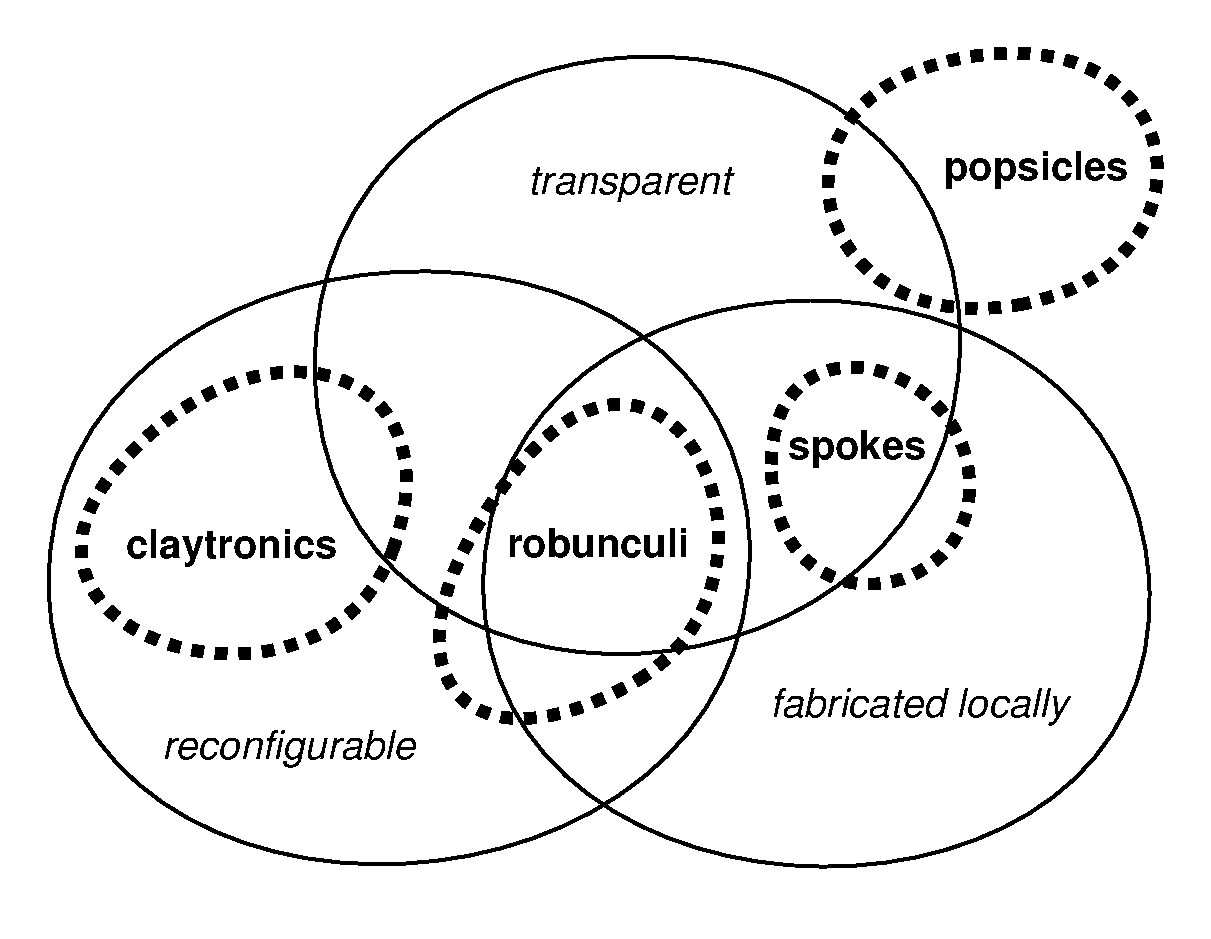
\includegraphics[width=120mm]{ecology_venn.pdf}
  \caption{Venn diagram showing which desiderata could be fulfilled by each responsive environment ecology.}
  \label{fig:ecology_venn}
\end{figure}

Of course several of these ecological niches may coexist, and influence each other. 
It seems that the only system capable of producing artifacts on a global scale in the near future is some kind of popsicle ecology. 
While ecologies dominated by popsicles may not support widespread participation as well as others, unless they are able to acquire responsive artifacts people will not be able to participate in responsive environments at all. 
For example the cell phone ecosystem is dominated by popsicles, and while cell phones are often not particularly transparent, they are broadly available almost everywhere%
\footnote{citation?}.
Even if popsicle ecosystems continue to dominate our ecology, developing spoke and robunculi ecosystems could place pressure on popsicles to support transparency and reuse (if not reconfiguration). 
We propose that our best opportunity for building an inclusive artifact ecology is to support the development of spokes and robunculi. 
Robunculi in particular can help to engage more people in design roles and help to scaffold participation in local fabrication scenes.

There are several potential advantages to adopting robunculi as the building blocks of our built environment: we could customize the form and behavior of the devices and structures around us; we could give many previously static objects the capacity to express behaviors; and we could decompose objects not currently in use to provide raw materials to be reused elsewhere. 
More significantly, robunculi have the potential to change the way we manipulate our environment much as googling has changed the way we gather information. 
With robunculi we can all be furniture{}-designing, golem{}-wrangling {\bf maker} cyborgs.

And as claytronic technologies mature, the ecologies developed by robunculi-wranglers could diverge significantly from those developed on top of popsicle ecologies with more limited opportunities for design input. 
Many of the methods currently being developed to support interacting with robunculi could be transferred to claytronic systems. 
Without this intermediate developmental stage claytronic systems may feature relatively impoverished mechanisms for encouraging input from those wielding (and inhabiting) these systems.

\section{Method and Goals}
%
Our current artifact ecologies provide extremely limited opportunities for people to participate in the design of their built environment. 
As we transition from leveraged to responsive environments the artifacts we surround ourselves with are being elevated from a variety of useful tools and spaces to cybernetic extensions of our personas. 
The question at hand then is: how we can live amongst robots in a way that empowers us to take control of the sorts of environments that ubiquitous computation will soon allow?

\subsection{Thesis}
%
\begin{em}
Robunculi ecologies empower people to control the behavior of the responsive environments they inhabit.
\end{em}

There are several features of these systems and their supporting ecology that make robunculi well suited to the development of engaged cybernetic communities. 
By supporting interaction methods that leverage our innate sensimotor capabilities robunculi make the specification of form and behavior accessible. By providing people with little training the opportunity to take on (relatively limited) design roles this ecology can scaffold skill development. 
And by developing an engaged community of skilled practitioners robunculi ecologies can serve as fertile ground for local scenes specializing in fabrication, software and hyperform behaviors.

\subsection{Method}
%
We support these claims by identifying these features in prototype robunculi systems currently being developed, first in a broad survey and then in several more focused case studies.
To facilitate this discussion we first develop (in Chapter~\ref{ch:ontology}) an ontology of responsive environments describing the roles we may adopt in relating to responsive artifacts, the interrelations between these roles and the methods of relation that typify each role. 
We devote particular detail to the roles and interaction methods supported by robunculi.

In Chapter~\ref{ch:survey} we survey responsive artifact prototypes from a variety of fields including tangible interfaces and modular robotics, with a focus on projects that satisfy our definition of robunculi. 
By describing them in terms of our ontology we call attention to the advantages of robunculi for supporting an engaged design ecosystem. 

In Chapter~\ref{ch:case_studies} we present case studies of several projects developed by the author and others in further detail.
We will focus on identifying reusable techniques and components of successful robunculi projects, on useful metrics for comparing the relative merits of different projects, and on how individual projects could relate to a larger ecosystem. 

We conclude in Chapter~\ref{ch:conclusion} with an assessment of the current state of robunculi development and directions for future research.




